\documentclass{article}
\usepackage[margin=8mm,paperwidth=26cm,paperheight=14cm]{geometry}
\usepackage{tikz}
\usetikzlibrary{arrows.meta,positioning,fit}
\pagestyle{empty}

\begin{document}
\thispagestyle{empty}
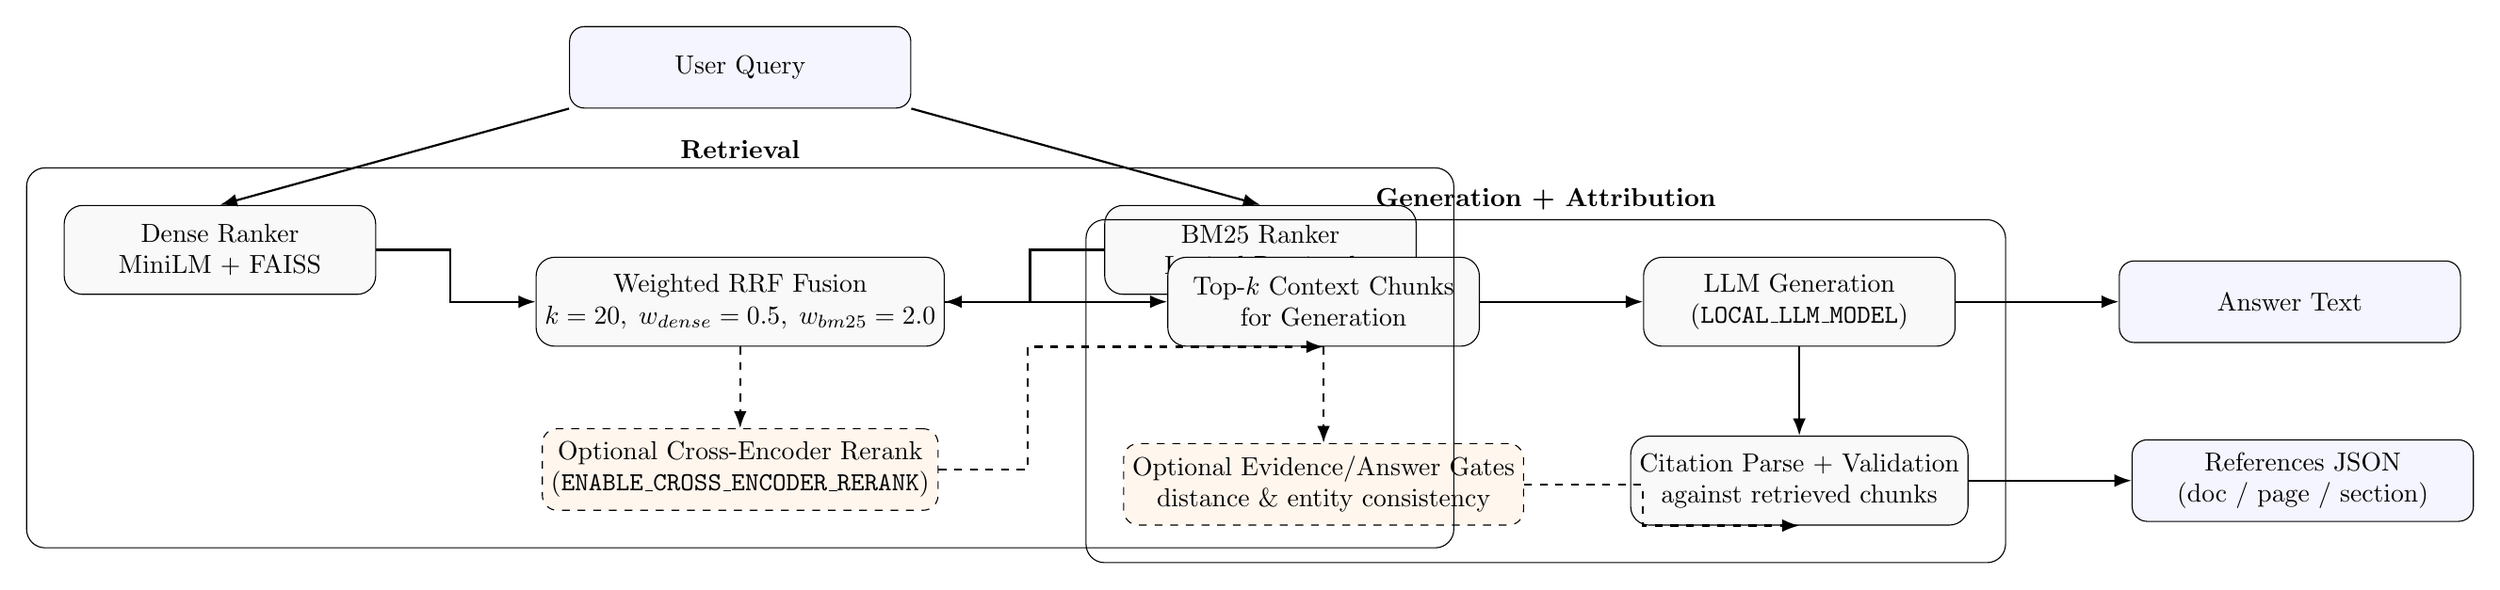
\begin{tikzpicture}[
    >=Latex,
    node distance=10mm and 14mm,
    box/.style={draw, rounded corners=2mm, minimum width=34mm, minimum height=11mm, align=center, fill=white},
    stage/.style={draw, rounded corners=2.5mm, minimum width=42mm, minimum height=12mm, align=center, fill=gray!5},
    io/.style={draw, rounded corners=2mm, minimum width=46mm, minimum height=11mm, align=center, fill=blue!4},
    optional/.style={draw, dashed, rounded corners=2mm, minimum width=42mm, minimum height=11mm, align=center, fill=orange!7},
    line/.style={->, thick},
    dline/.style={->, thick, dashed}
]

% Query + retrieval branches
\node[io] (q) {User Query};
\node[stage, below left=13mm and 26mm of q] (dense) {Dense Ranker\\MiniLM + FAISS};
\node[stage, below right=13mm and 26mm of q] (bm25) {BM25 Ranker\\Lexical Retrieval};

\draw[line] (q.south west) -- (dense.north);
\draw[line] (q.south east) -- (bm25.north);

% Fusion + rerank
\node[stage, below=20mm of q] (rrf) {Weighted RRF Fusion\\$k=20,\;w_{dense}=0.5,\;w_{bm25}=2.0$};
\draw[line] (dense.east) -- ++(10mm,0) |- (rrf.west);
\draw[line] (bm25.west) -- ++(-10mm,0) |- (rrf.east);

\node[optional, below=11mm of rrf] (ce) {Optional Cross-Encoder Rerank\\(\texttt{ENABLE\_CROSS\_ENCODER\_RERANK})};
\draw[dline] (rrf) -- (ce);

% Context + generation
\node[stage, right=30mm of rrf] (ctx) {Top-$k$ Context Chunks\\for Generation};
\draw[line] (rrf.east) -- (ctx.west);
\draw[dline] (ce.east) -- ++(12mm,0) |- (ctx.south);

\node[stage, right=22mm of ctx] (llm) {LLM Generation\\(\texttt{LOCAL\_LLM\_MODEL})};
\draw[line] (ctx.east) -- (llm.west);

% Validation/citations/output
\node[stage, below=12mm of llm] (val) {Citation Parse + Validation\\against retrieved chunks};
\draw[line] (llm.south) -- (val.north);

\node[io, right=22mm of llm] (ans) {Answer Text};
\node[io, right=22mm of val] (cit) {References JSON\\(doc / page / section)};
\draw[line] (llm.east) -- (ans.west);
\draw[line] (val.east) -- (cit.west);

% Optional gating
\node[optional, below=13mm of ctx] (gate) {Optional Evidence/Answer Gates\\distance \& entity consistency};
\draw[dline] (ctx.south) -- (gate.north);
\draw[dline] (gate.east) -- ++(16mm,0) |- (val.south);

% Group boxes
\node[draw, rounded corners=2.5mm, fit=(dense)(bm25)(rrf)(ce), inner sep=5mm, label={[font=\bfseries]above:Retrieval}] {};
\node[draw, rounded corners=2.5mm, fit=(ctx)(llm)(val)(gate), inner sep=5mm, label={[font=\bfseries]above:Generation + Attribution}] {};

\end{tikzpicture}
\end{document}
